\chapter{Results and Discussion} \label{Results}
\section{Results} \label{Results}
Results obtained from the implementation of FIS in MATLAB are compared with the implemented code and the outputs are verified
\subsection{Case1} \label{Case 1: 3 metrics}
\begin{figure}[H]
\centering
\subfigure[Stage 1 fuzzification outputs]
	{
	\label{fig:a}
	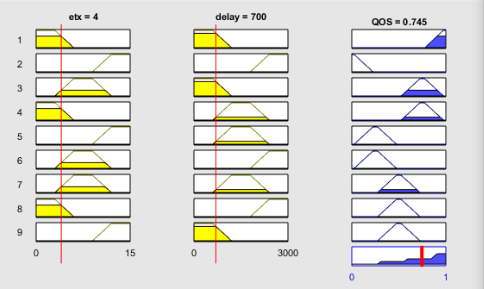
\includegraphics[width=100mm]{MATLAB3inputsa.png}
	}
\subfigure[Stage 2 fuzzification outputs]
	{
	\label{fig:b}
	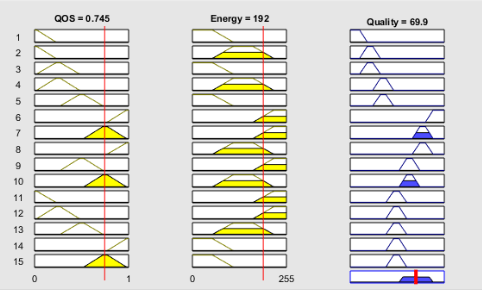
\includegraphics[width=100mm]{MATLAB3inputsb.png}
	}
\caption{results of Fuzzy controller in MATLAB for 3 inputs}
\label{fig:method}
\end{figure}
\begin{figure}[h!]
\centering
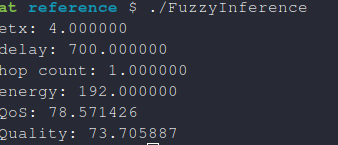
\includegraphics[width=50mm]{result3inputcode.png}
\caption{result from c implementation}
\end{figure}

\subsection{Case 2} \label{Case 2: 4 metrics}
\begin{figure}[H]
\centering
\subfigure[Stage 1 fuzzification outputs]
	{
	\label{fig:a}
	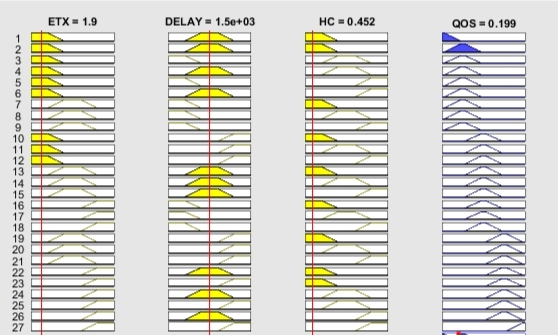
\includegraphics[width=100mm]{MATLAB4inputsa.jpeg}
	}
\subfigure[Stage 2 fuzzification outputs]
	{
	\label{fig:b}
	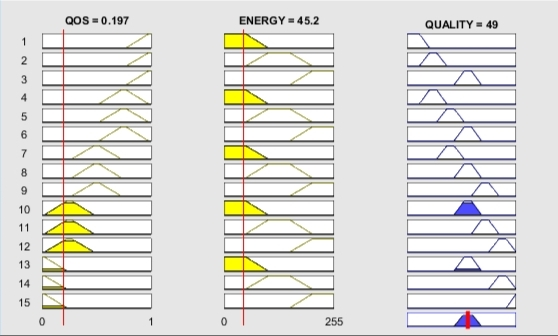
\includegraphics[width=100mm]{MATLAB4inputsb.jpeg}
	}
\caption{results of Fuzzy controller in MATLAB for 4 inputs}
\label{fig:method}
\end{figure}
\begin{figure}[h!]
\centering
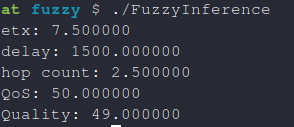
\includegraphics[width=50mm]{result4inputcode.png}
\caption{result from c implementation}
\end{figure}
\section{Discussion} \label{Discussion}
To more precisely test the extent of the influence of Delays/Latency and Jitter in the Optimised Network we will have to carry out simulations for longer durations of time(1hr, 10hrs, 20hrs).
We may also carry out the simulations using the optimised routing protocol for larger networks which may comprise of a few hundreds of nodes.
We may also test the various existing OFs which use Fuzzy Logic for metrics combination with the OF we have designed.
